\chapter{AFIDs-Pred: Stereotactic Target Localization Using Anatomical Fiducials}\label{chap:afidspred}
\newpage
\sloppy
\noindent This chapter is largely based on:
\begin{itemize}[noitemsep,topsep=0pt]
    \begin{small}
    \item
    A. Taha, M. Abbass, M. Snyder, D. Bansal, J. Zhao, E. Coskun, V. Liu, G. Gilmore, A.R. Khan, J.C. Lau.
    \end{small} Optimizing indirect localization of deep brain targets using anatomical fiducials and machine learning. \textit{In Preparation}.
\end{itemize}


\section{Introduction}

\subsection{Stereotaxy and modern neuroimaging}
The origins of coordinate-based brain mapping can be traced back to Horsley and Clarke \cite{Horsley1908-om}, who designed a stereotaxic apparatus using Cartesian coordinates to localize brain structures relative to cranial landmarks. Building on this foundation, Jean Talairach \cite{Schaltenbrand1977-ge, Talairach1957-eb} leveraged anatomical landmarks, such as the anterior commissure (AC) and posterior commissure (PC), for more refined brain structure localization (i.e., the proportional grid normalization). These early innovations laid the groundwork for population-based brain templates that emerged with the advent of MRI. For example, the MNI305 template \cite{Collins1994-dx} aligned 305 individual MRI scans using AC and PC, overcoming the idiosyncrasies of using a single subject brain as a template. Subsequent advances in non-linear registration further refined these templates, culminating in modern standards such as the MNI152 space \cite{Fonov2009-oi}, now widely employed for aligning anatomical data. Despite these advances, localizing small, poorly visualized structures with millimetric accuracy remains a challenge, particularly when direct anatomical visualization is limited by image resolution, contrast, or artifacts (see Section \ref{sec:SNSX} for a detailed overview).

\subsection{Millimeters Matter in Deep Brain Stimulation}
Deep brain stimulation (DBS) is a stereotactic procedure involving the surgical implantation of electrodes in specific brain structures (see Section \ref{sec:whymm} for a more detailed overview). It is well established for the management of a wide array of movement disorders such as Parkinson's disease (PD), essential tremor, dystonia, and Tourette’s syndrome, as well as for select psychiatric conditions including obsessive-compulsive disorder and treatment-resistant depression \cite{Lozano2019-dv}. In the case of movement disorders, small deviations in electrode position during DBS result in side-effects including paresthesias, pyramidal symptoms, diplopia, and dysarthria \cite{Buhmann2017-da}. Meanwhile, sub-optimal placement of the electrode on the order of 2 millimeters (mm) can lead to reduced clinical outcomes \cite{Horn2019-by} and put patients at risk for post-operative cognitive decline \cite{Reich2022-jf}.

\subsection{Challenges in Localizing DBS Targets}
Achieving the level of precision needed in DBS is complicated by the limitations of clinical neuroimaging. Most MRI scanners used in clinical settings operate at 1.5 or 3 T, which may not always provide the resolution required to clearly visualize small DBS targets such as the STN. Furthermore, patient motion—exacerbated in individuals with movement disorders—suboptimal MRI protocols, and geometric distortions can further degrade image quality \cite{Boutet2021-vg, Chandran2016-eg, Lau2018-fp}. Ultra-high field (UHF; $\geq$7T) MRI enables clear delineation of small brain regions, since increased magnetic field strength yields enhanced signal-to-noise ratio and tissue contrast that can be exploited to improve spatial resolution \cite{Abosch2010-jn, Duchin2012-db, Lau2017-ea, Lau2020-dh, Lenglet2012-ii}. However, UHF-MRI systems are not commonly available, limiting widespread clinical adoption \cite{Clarke2020-ky}. As a result, DBS targeting may employ indirect localization techniques that rely on predefined coordinate spaces.

\subsection{Indirect Brain Target Localization Approaches}
Existing methods for indirect localization can be grouped into two categories: (1) atlas-based consensus coordinates and (2) atlas-based registration. Atlas-based coordinate approaches describe consensus coordinates of a target relative to the midpoint along the AC-PC line, known as the mid-commissural point (MCP). The MCP is susceptible to intersubject variability, as no single atlas-based consensus coordinate perfectly captures the anatomical differences observed across populations. Meanwhile, atlas-based (i.e., deformable) registration techniques estimate the deformation field used to propagate atlas labels from a stereotactic space (e.g., MNI) to individual brains. Deformable registration yields errors on the order of 1-5 mm \cite{Lau2019-eh, Abbass2022-lf, Miller2023-ct}, with lower quality clinical scans prone to failing thus requiring manual intervention. Furthermore, surgical planning often occurs on gadolinium enhanced T1w scans (MRI-gad), to ensure safe implantation of electrodes while avoiding blood vessels, introducing further complexity to the  registration process \cite{Abbass2022-lf, Abbass2025-el} and application of standard neuroimaging workflows which may not be optimized for MRI-gad \cite{Ogunsanya2024-uf, Warntjes2014-wy}.

\subsection{Machine Learning for Automatic Brain Target Localization}
Machine learning (ML) models for automatic localization of brain structures have gained significant interest offering a faster and more generalizable alternative to deformable registration \cite{Baniasadi2023-lm, Ren2025-zu}. However, only a limited number of studies evaluated and adapted ML frameworks to the small DBS targets while achieving generalizability on clinical quality (e.g., MRI-gad) scans \cite{Baniasadi2023-lm}. Furthermore, due to the intensive process of acquiring manual ground-truth labels, many approaches have focused on matching accuracy of well-curated parameters during deformable registration approaches (i.e., training labels generated from quality controlled deformable registration segmentation data) \cite{Baniasadi2023-lm}.

\subsection{Coordinate-to-Coordinate Machine Learning Framework}
In this study, we validate an ML framework to accurately localize brain structures solely from $x$, $y$, $z$ coordinates of surrounding anatomical landmarks (i.e., coordinate-to-coordinate). Our target localization approach is dependent only on validated anatomical landmarks inspired from classical stereotactic methods \cite{Lau2019-eh, Abbass2022-lf}, which are reproducible across various MRI field strengths and modalities (see Chapter \ref{chap:afidsdata}). This framework was designed with generalizability and explainability in mind, such that it can be applied to other brain targets while enabling understanding of relationships between predefined landmarks and the targeted brain region, including structures targeted in DBS (i.e., STN). Our framework integrates well within the clinical workflow, which already involves preoperative localization of landmarks (e.g., AC and PC). Central to our approach is an open-source framework, which involves the release of our coordinate data, code, and our framework in the form of a website \url{https://stereotaxy.afids.io}.

\begin{figure}[hbt!]
    \centering
    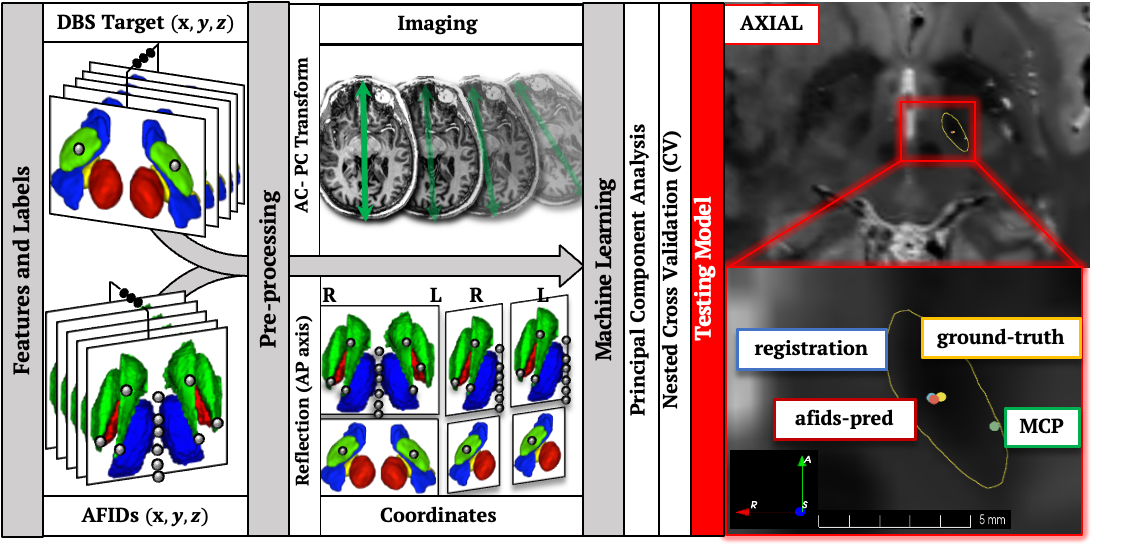
\includegraphics[width=0.9\linewidth]{figs/ch4_Figure_afidspred.png}
    \caption{Overall workflow for building our machine learning (ML) model to localize the subthalamic nucleus (STN) using anatomical fiducials (AFIDs). Validated AFID coordinates were used as features to predict STN coordinates. All coordinates were anterior commissure (AC) and posterior commissure (PC) aligned. AFID and STN coordinates on the right hemisphere were mirrored to augment data. Principal component analysis (PCA) was performed on coordinate data to capture collinearity. A nested 4-fold cross validation strategy was employed for ML training. Model prediction was validated on various imaging modalities and compared to deformable registration for STN localization.}
    \label{fig:ch4_Figure_afidspred}
\end{figure}

\section{Methods}

\subsection{Participants}
We leverage 202 MRI scans on which we have more than 6,500 ground truth anatomical landmarks applied in accordance with a validated annotation protocol \cite{Lau2019-eh} by more than 20 human raters (Table \ref{tab:afidpred_datasets}). Although this data set has been described previously in Chapter \ref{chap:afidsdata}, we divide them below to emphasize their different use cases in this chapter. 

The Stereotactic Neurosurgery (SNSX) dataset. This dataset consists of 61 participants (32 healthy controls and 30 scheduled for DBS). Participants were imaged using a 7T head-only MRI scanner (Siemens Magnetom; Siemens Healthineers, Erlangen, Germany) at the Center for Functional and Metabolic Mapping (CFMM) in Western University (REB: 109045). The MRI sequences used for this study were: 1) 3D T1w MP2RAGE and 2) 3D optimized T2w fast-spin echo (T2 SPACE).

The London Health Sciences Center Parkinson’s Disease (LHSCPD) dataset. This dataset consists of a subset (n = 10) of the same participants as in the SNSX dataset, scheduled to undergo DBS at London Health Sciences Center (LHSC; REB: R-17-156). Participants were imaged using a 1.5T MRI scanner (Signa, 1.5T, General Electric, Milwaukee, Wisconsin, USA). The MRI sequence used in this study was a 3D T1w MP2RAGE with gadolinium contrast (termed “MRI-gad” in subsequent sections).

An openly released 3T and 7T (3T-7T) dataset \cite{Chen2023-cn}, consisting of healthy participants (n = 10) imaged using the following sequences: 1) 3D T1w MP2RAGE and 2) 3D T2 SPACE. Participants are imaged at both 3T and 7T (i.e., test-retest).

A subset of a previously released dataset (afids-data; see Chapter \ref{chap:afidsdata}) dataset, which aggregated landmark annotations (n = 110) on various populations (healthy, abnormal ventricular size, and PD). The participants in this subset are independent of the previously mentioned datasets.

\subsection{Coordinate Data Annotation}
We employ a previously validated protocol for the annotation of anatomical fiducials (AFIDs; \url{https://afids.github.io/afids-protocol}) providing a point-based sampling of multiple brain structures. In this study, we selected a subset of 16 AFIDs (available on \url{https://stereotaxy.afids.io}) described by the protocol that: (1) circumscribe the midbrain and surrounding structures (e.g. DBS targets) and (2) can be localized within 1 mm.

\begin{table}[h!]
\centering
\caption{Various datasets leveraged as part of this study, all of which have curated anatomical landmark annotations.}
\begin{tabularx}{\textwidth}{l l l l l}
\toprule
\textbf{Dataset} & \textbf{Field Strength (T)} & \textbf{Disease (n)} & \textbf{Analysis} \\
\midrule
SNSX* & 7 & HC (32), PD (30) & Training and Testing  \\
LHSCPD & 1.5 (paired SNSX) & PD (10) & Clinical Validation \\
3T-7T* & 3 and 7 (paired) & HC (10) & External Validation  \\
afids-data & 1.5, 3, and 7 & HC (60), PD (40), AD (10) & Landmark Generalization \\
Template & 3 & HC (1) & Landmark Augmentation  \\
\bottomrule
\end{tabularx}

\vspace{1ex}
\raggedright
\footnotesize{
\textbf{HC} = healthy control, \textbf{PD} = Parkinson’s disease, \textbf{AD} = Alzheimer’s disease.\\
* Contains manual human rater curated subthalamic nucleus (STN) segmentations.
}
\label{tab:afidpred_datasets}
\end{table}

\textbf{AFID Annotations:} All annotations were performed in accordance with the AFIDs protocol via 3DSlicer 4.10. Rater placements per AFID were averaged to curate the ground-truth coordinates ($x$, $y$, $z$).

\textbf{STN Annotations:} All annotations were performed via 3DSlicer 4.10 \cite{Fedorov2012-rk} using the smallest configuration of the paint brush (1 mm) and the pencil drawing tool on 7T T2w imaging. Rater segmentations per subject were selected via majority voting (\(>\)50\%) and then collapsed to a center of mass representing the STN centroid, constituting the ground truth STN centroid coordinates ($x$, $y$, $z$).

Each scan was annotated by at least two human raters (see Supplementary section \ref{app:rater_demo_data} for a breakdown of rater demographic data). The ground truth coordinates were quality controlled (QC) by three raters (AT, JZ, and EC). We provide example QC files (Supplementary Section \ref{app:qualitycontrol}) with accompanying code and ground truth coordinates (*.fcsv) used in this work on: \url{https://github.com/afids/afids-pred}.

\subsection{Coordinate Data Processing}
An AC-PC alignment was performed followed by centering coordinates at the mid-commissural point (MCP; defined as the midpoint between AC and PC). Coordinates on the left hemisphere were reflected to the right by inverting the sign of the x-coordinate after AC-PC transformation and MCP centering. Thus, each participant constituted two augmented examples. Preliminary analysis using training data was conducted to investigate correlations across coordinates to inform ML. Subsequently, principal component analysis (PCA) was performed on concatenated x, y, z coordinates. Top principal components (PCs) capturing 99\% of the variance were retained for subsequent ML model training.

\subsection{Data Split and Machine Learning}\label{chap:afidspredML}
AFID and STN coordinate data of participants from the SNSX dataset were used for ML training. Ten participants from the SNSX dataset were assigned to a reserved testing dataset used solely to report the accuracy of our model. These participants were also the same ones from the LHSCPD dataset, enabling evaluation of our model on clinical quality 1.5T MRI-gad scans. Finally, the 3T-7T dataset was used for external validation to report prediction accuracy at 3T and 7T MRI.

To explore the trade-off between model simplicity and complexity, we evaluated two ML algorithms: (1) \textit{Ridge Regression} \cite{Hoerl1970-so}, a linear model with built-in regularization, and (2) \textit{Extreme Gradient Boosting} (XGBoost; \cite{Friedman2001-hp}), an ensemble-based method capable of modeling non-linear relationships. 

ML models were trained via a nested cross-validation (CV) strategy to tune hyperparameters and evaluate performance (scikit-learn; \cite{Pedregosa2012-ab}). The outer CV loop involved a 4-fold split of all training data for statistically evaluating the two ML models, and the inner CV loop involved a 3-fold split CV strategy for tuning hyperparameters. All the folds were curated such that for a given training example (i.e., participant) the left and right hemisphere target labels (e.g., STN) were grouped together. This prevented a scenario where the left and right labels appear separately across training and testing to avoid data leakage. Furthermore, group based preprocessing (i.e., PCA) was performed independently within each fold to prevent leakage across folds. Final model accuracy was reported on the four testing sets curated by the outer CV loops. We compute the x, y, z mean squared error (MSE) and Euclidean distance (ED) to evaluate models. See Figure~\ref{fig:ch4_Figure_afidspred} for an end-to-end abstraction of our methodology.

\subsection{Model Robustness, Generalizability, and Comparative Evaluation}

\textbf{Generalization to Other Imaging Modalities.} To investigate model accuracy on clinical-grade imaging, STN coordinate predictions on 1.5-T MRI-gad scans were statistically compared to paired ground-truth counterpart 7-T MRI-nogad scans. To further demonstrate robustness across research-grade imaging and external data, we also evaluated model predictions on the 3T–7T dataset. Statistical comparisons were in AC-PC space and two independent Wilcoxon signed-rank tests were performed across $x$,$y$,$z$ MSE and ED with Bonferroni correction ($\alpha = 0.05 / 4$).

\textbf{Benchmarking.} We perform statistical comparisons between our model and deformable registration for STN localization using our 1.5T MRI-gad dataset (i.e., LHSCPD) and paired 7T-MRI counterpart (i.e., SNSXPD). The Distal atlas segmentations in MNI space \cite{Chakravarty2006-ln, Ewert2018-bn} were warped to native space using presets from a nonlinear deformation framework validated via 11,000 non-linear warps across more than 100 subjects \cite{Ewert2019-cc}. We apply this framework as implemented in Lead-DBS software (v.3.1; \cite{Neudorfer2023-wd}). Groups were compared using a signed-Wilcoxon Rank Test.

\textbf{Robustness to Annotation Variability.} To investigate model dependency on accurate localization, we make use of 38 independent AFID protocol applications in a common space (i.e., MNI) and evaluate STN prediction accuracy across these trials. For this analysis, the AFID protocol was applied independently by 10 human raters. 

\textbf{Generalizability to Other Brain Landmarks.} To investigate the generalizability of our framework to other brain landmarks, we iteratively drop each brainstem AFID (i.e., leave-one-AFID out) and predict it using the other AFIDs. This analysis was conducted using all the datasets (i.e., n = 202) for nine AFIDs and employed the same nested-cross validation approach described in section \ref{chap:afidspredML}.

\subsection{Model Deployment}
Building on the previous open software infrastructure of the AFID project, we deploy our model on a website (\url{https://stereotaxy.afids.io}). This enables users to upload their AFID placements as specified by our protocol and receive STN coordinate predictions alongside an AC-PC transformation matrix. Additionally, we also deploy our STN prediction model within a larger suite of coordiante-based tools (i.e., \texttt{AutoAFIDs}; see Chapter \ref{chap:AutoAFIDs}) which automatically localizes AFIDs from MRI volume. Details about running the end-to-end workflow (i.e., image to DBS target) is presented in Supplementary content \ref{app:stereotaxyautoafids}. For subsequent sections, we report the results and discuss them independently of \texttt{AutoAFIDs} for completeness. 

\section{Results}

\subsection{Rater Curated Data}
The localization error across all AFID placements and datasets was 0.84~$\pm$~0.31~mm. The inter-rater STN segmentation overlap was 0.78~$\pm$~0.03, measured using the Dice similarity coefficient. There was no statistical difference between right and left hemisphere STN segmentations, thus they were combined in subsequent descriptive summaries. The average volumes of the STN for the healthy control (HC) and Parkinson’s disease (PD) cohorts were 136.56~$\pm$~16.24~mm\textsuperscript{3} and 128.03~$\pm$~29.67~mm\textsuperscript{3}, respectively ($p = 0.047$; Mann–Whitney U test). The average x, y, z STN coordinates in MCP space for the HC and PD cohorts were: 10.18, -0.92, -3.27 and 10.14, -0.88, -3.61, respectively (x: $p = 0.93$, y: $p = 0.91$, z: $p = 0.002$; Mann–Whitney U test). Only the z-coordinate was statistically significant after Bonferroni correction ($\alpha = 0.05/4$).

\subsection{Preliminary Analysis and Principal Component Analysis}
Pairwise correlations were computed among the x, y, and z coordinates of 16 AFIDs (48 features total) across training data (see Figure~\ref{fig:ch4_Figure_PCA}a). Principal component analysis (PCA) was employed to reduce the dimensionality of features used for ML model training. The top 23 principal components (PCs) captured 99\% of the variation in the data (see Figure~\ref{fig:ch4_Figure_PCA}b) and were chosen for subsequent analysis. Further exploration of AFID contributions to PCs revealed relatively broad AFID contributions (see Figure~\ref{fig:ch4_Figure_PCA}c). Strong linear associations between AFID coordinates and STN x, y, and z coordinates were observed (Pearson’s r = -0.38–0.54) in the training data (see Figure~\ref{fig:ch4_Figure_stncor}), supporting the use of a linear regression framework.

\begin{figure}[hbt!]
    \centering
    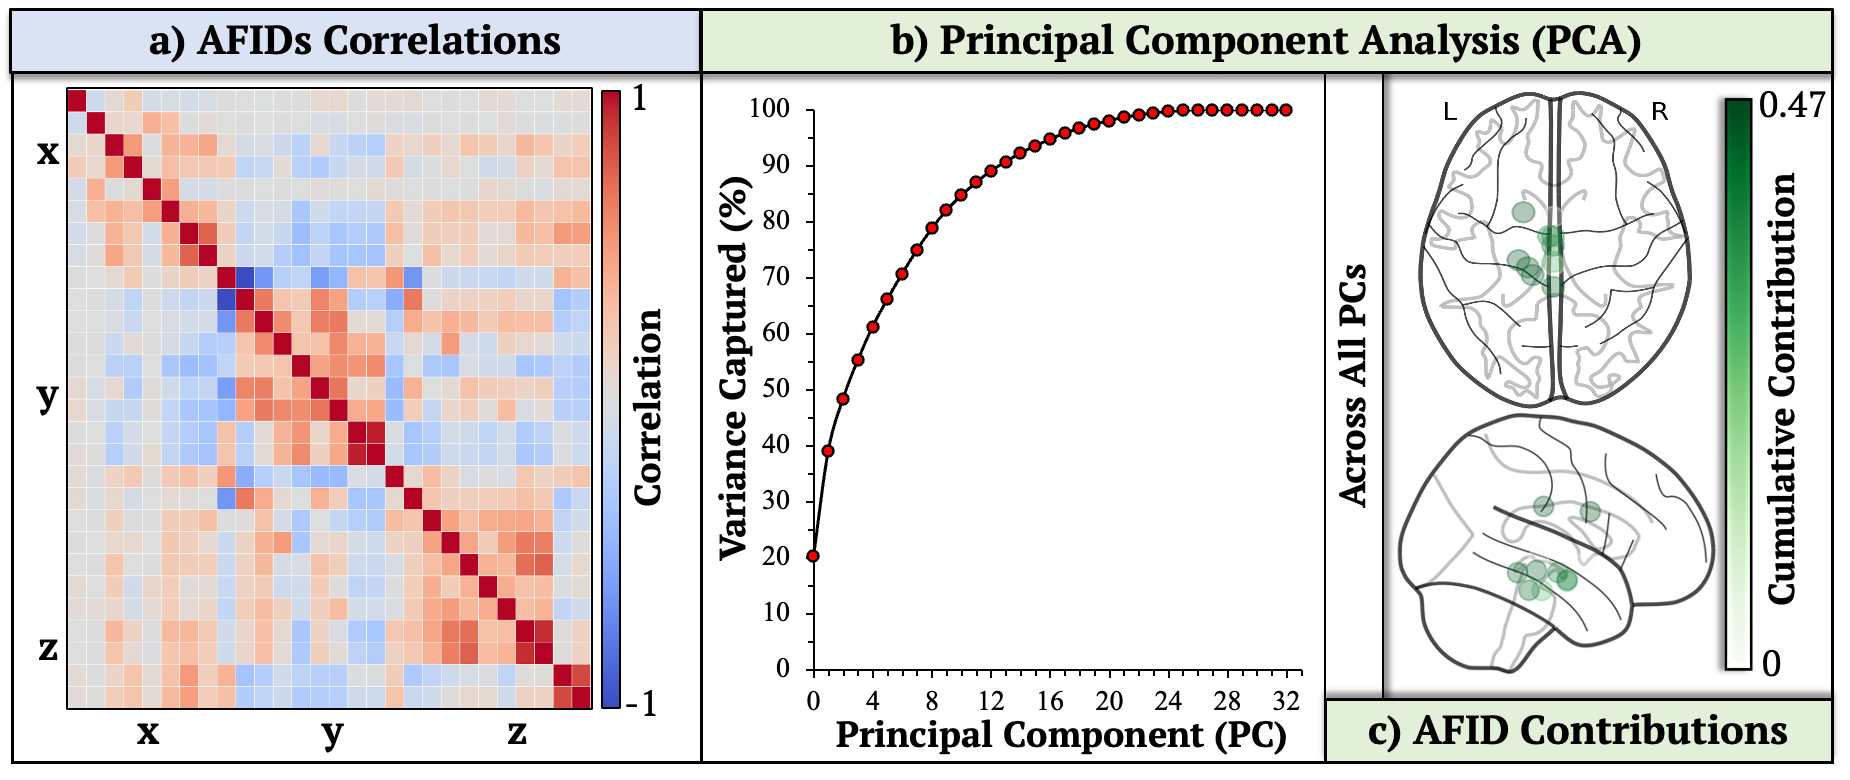
\includegraphics[width=1\linewidth]{figs/ch4_Figure_PCA.png}
    \caption{Correlation and visual representation of landmarks and Principal Component Analysis (PCA). a) Correlation matrix between the x, y, and z coordinates of anatomical fiducials (AFIDs) chosen to build the machine learning model, post anterior and posterior commissure (AC-PC) transformation and mid-commissural point (MCP) centering. b) Cumulative explained variance plot as a function of principal components (~99\% of the variation with 24 components). c) Shows the weight contribution of each AFID’s x, y, and z coordinates to all principal components.}
    \label{fig:ch4_Figure_PCA}
\end{figure}

\subsection{Machine Learning Model Performance}
\textbf{Model Training:} A multi-output paradigm using nested CV was used to train a ridge regressor and an XGBRegressor. ED computed on the outer CV folds was compared using a Wilcoxon signed-rank test, and the ridge regressor statistically outperformed the XGBRegressor ($\alpha = 0.05$, $p < 0.01$), supporting its use as the final model for predicting STN coordinates.

\begin{figure}[hbt!]
    \centering
    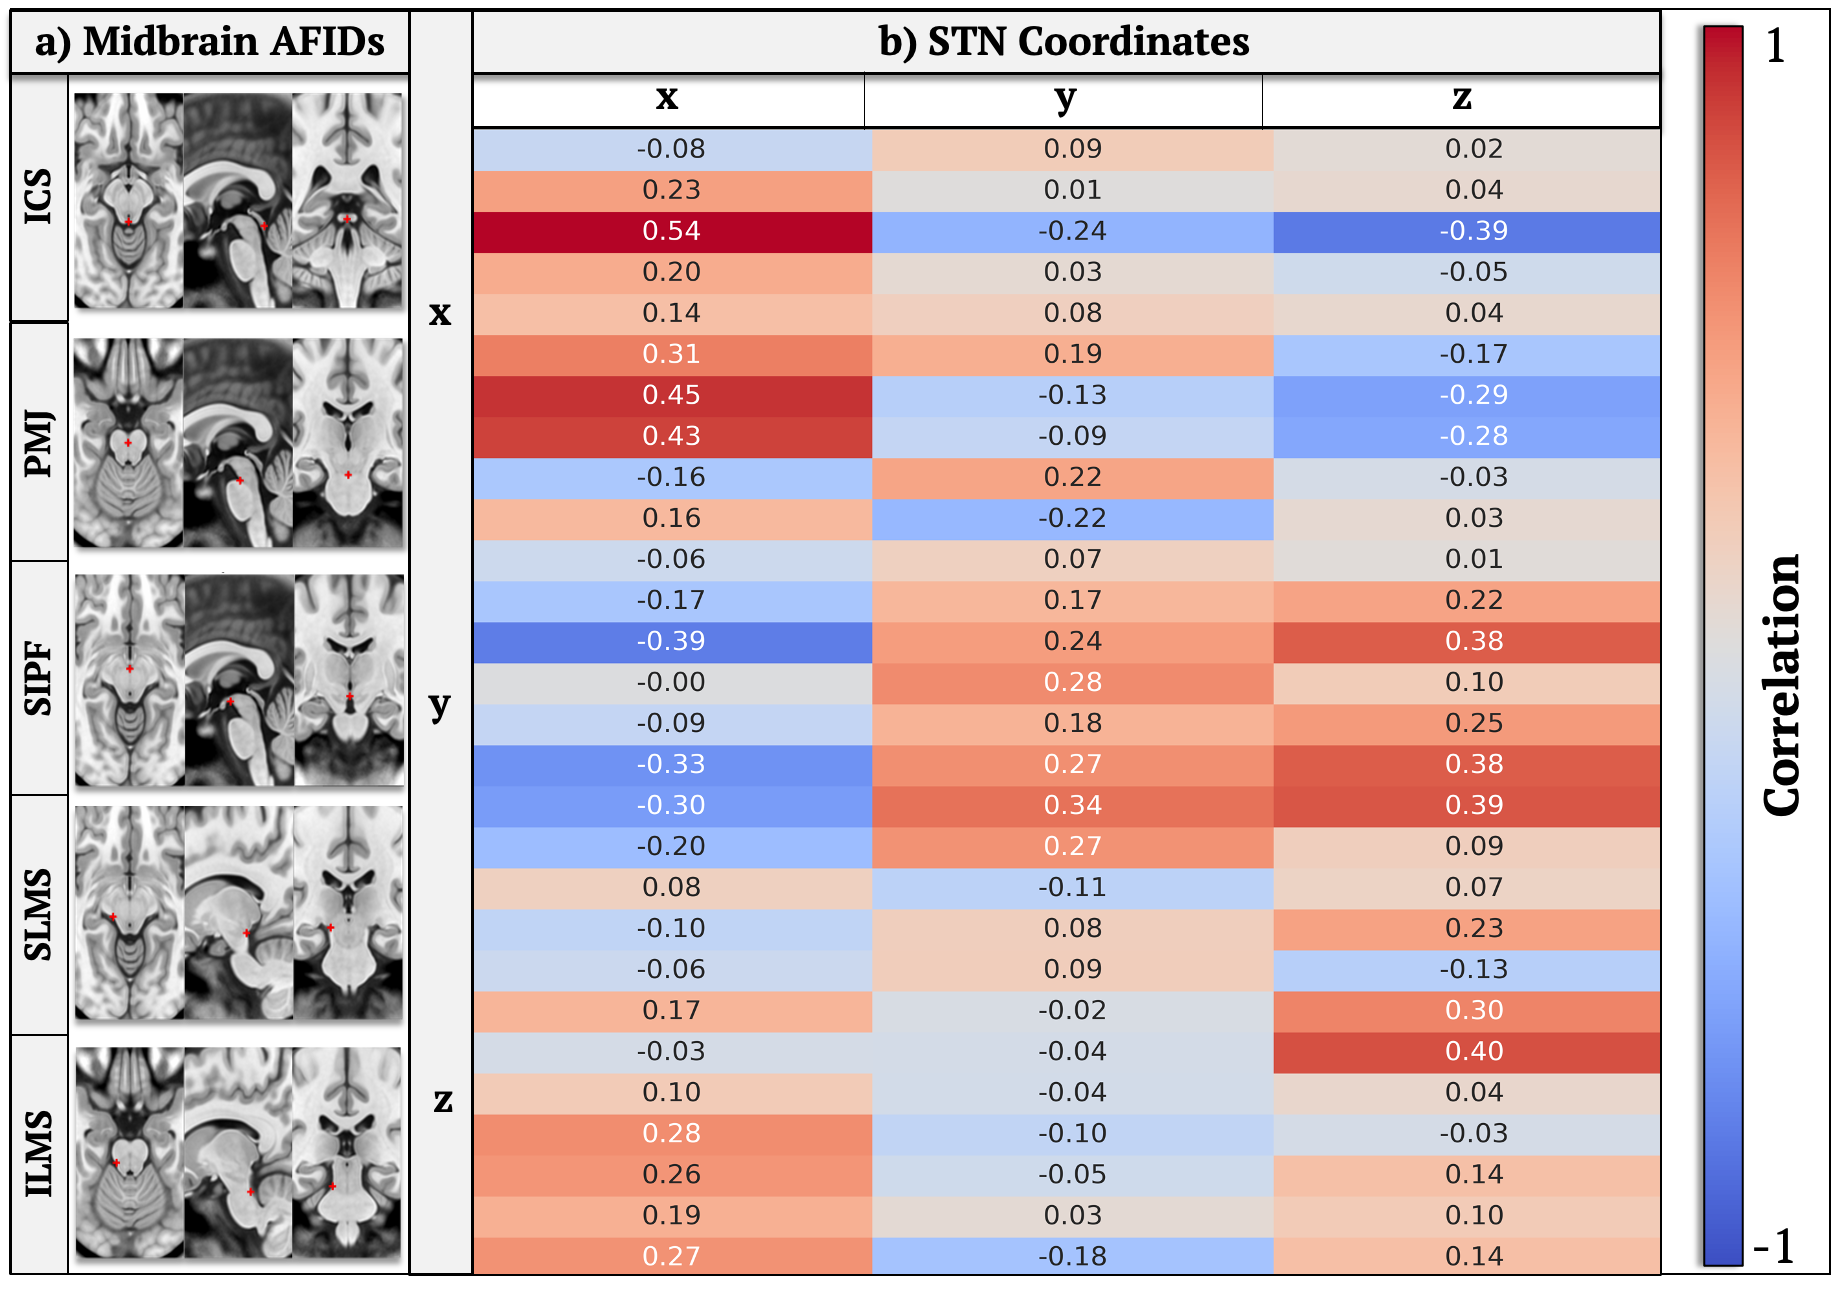
\includegraphics[width=1\linewidth]{figs/ch4_Figure_stncor.png}
    \caption{Correlation matrix of anatomical fiducials (AFIDs) and subthalamic nucleus (STN) coordinates. a) shows a subset of five AFIDs in the three cardinal planes which closely circumscribe the STN for anatomical context. b) Strong linear associations between x,y,z components of AFIDs and x,y,z dimensions of STN center of mass. }
    \label{fig:ch4_Figure_stncor}
\end{figure}

\textbf{Model Testing:} The average x, y, z mean squared errors (MSE) across all testing data (40 STNs) were: 0.45~$\pm$~0.56~mm, 0.66~$\pm$~0.79~mm, and 0.48~$\pm$~0.58~mm, respectively. The overall median ED error was 1.20~$\pm$~0.44~mm (IQR: 0.84–1.52). See Table~\ref{tab:performance_metrics} for a more granular breakdown of results.

\begin{table}[htbp]
\centering
\small
\caption{Performance of the final machine learning model across test datasets. Values are reported as Median ± Standard Deviation [Interquartile Range] for each dataset. Metrics include mean squared error (MSE) in the $x$, $y$, and $z$ directions, and Euclidean distance (ED).}
\label{tab:performance_metrics}
\begin{tabularx}{\textwidth}{lXXXX}
\toprule
\textbf{Dataset} & \textbf{MSE (x)} & \textbf{MSE (y)} & \textbf{MSE (z)} & \textbf{ED} \\
\midrule

\textbf{Testing Data (SNSX)} & 
0.48 ± 0.48 [0.22–0.88] & 
0.30 ± 0.77 [0.08–0.76] & 
0.43 ± 0.38 [0.03–0.72] & 
1.19 ± 0.37 [0.98–1.50] \\

\textbf{Clinical Validation (LHSCPD)} & 
0.24 ± 0.58 [0.09–0.68] & 
0.80 ± 0.87 [0.08–0.93] & 
0.57 ± 0.58 [0.11–0.79] & 
1.32 ± 0.42 [1.07–1.58] \\

% \textit{p}-value (SNSX vs LHSCPD) & 
% 0.13 (ns) & 
% 0.09 (ns) & 
% 0.11 (ns) & 
% 0.12 (ns) \\

\cmidrule(l){1-5}

\textbf{External Validation (3T)} & 
0.10 ± 0.57 [0.05–0.44] & 
0.43 ± 0.76 [0.06–1.30] & 
0.07 ± 0.78 [0.02–0.65] & 
1.20 ± 0.49 [0.80–1.49] \\

\textbf{External Validation (7T)} & 
0.07 ± 0.60 [0.02–0.27] & 
0.26 ± 0.78 [0.04–0.93] & 
0.17 ± 0.57 [0.03–0.49] & 
1.08 ± 0.48 [0.70–1.40] \\

% \textit{p}-value (3T vs 7T) & 
% 0.21 (ns) & 
% 0.31 (ns) & 
% 0.52 (ns) & 
% 0.15 (ns) \\

\bottomrule
\end{tabularx}
\end{table}

\subsection{Model Generalizability and Comparisons}

\textbf{Validation across Other Imaging Modalities:} We evaluated model performance across different imaging modalities by analyzing paired datasets acquired at various field strengths (see Figure~\ref{fig:ch4_Figure_errs}). Ten participants with both 1.5T MRI-gad (LHSCPD) and 7T MRI-nogad (SNSX), as well as ten participants with both 3T and 7T MRI (3T-7T), were included (see Section \ref{chap:afidspredML}). Wilcoxon signed-rank test with Bonferroni correction ($\alpha = 0.05/4$) revealed no significant differences in x, y, z MSE and ED across the two paired imaging modalities.

\begin{figure}[hbt!]
    \centering
    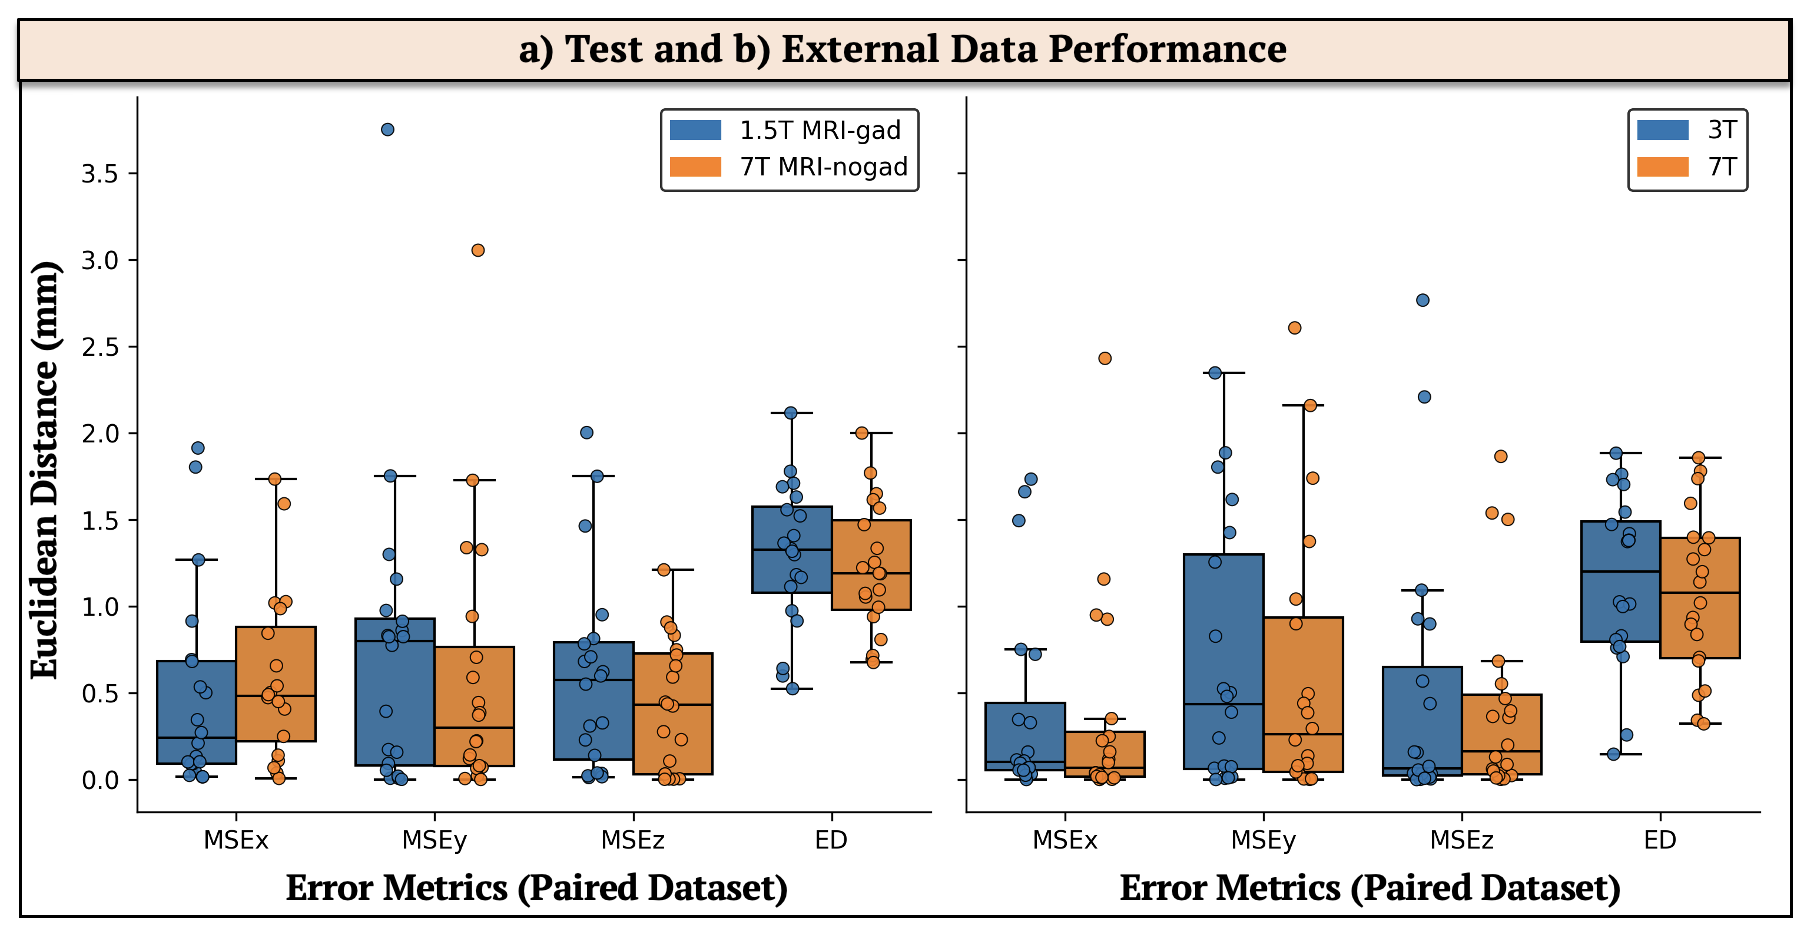
\includegraphics[width=1\linewidth]{figs/ch4_Figure_errs2.png}
    \caption{Model Performance on MRI modalities of Test-retest Datasets. a) shows model performance on 1.5T MRI with gadolinium (gad) and 7T MRI without gadolinium. b) shows model performance on 3T and 7T MRI. p \(>\) 0.1 across all axes and Euclidean distance. }
    \label{fig:ch4_Figure_errs}
\end{figure}

\textbf{Model Comparison and Performance Benchmarking:} We benchmarked our model against deformable registration (see Figure~\ref{fig:ch4_Figure_bench}a). On 1.5T MRI-gad scans, our model statistically outperformed registration ($p < 0.001$). Conversely, on multispectral 7T MRI-nogad data (i.e., registration warps computed using both T1 and T2 imaging), no significant difference in performance was observed between registration and our model ($p > 0.1$).

\begin{figure}[hbt!]
    \centering
    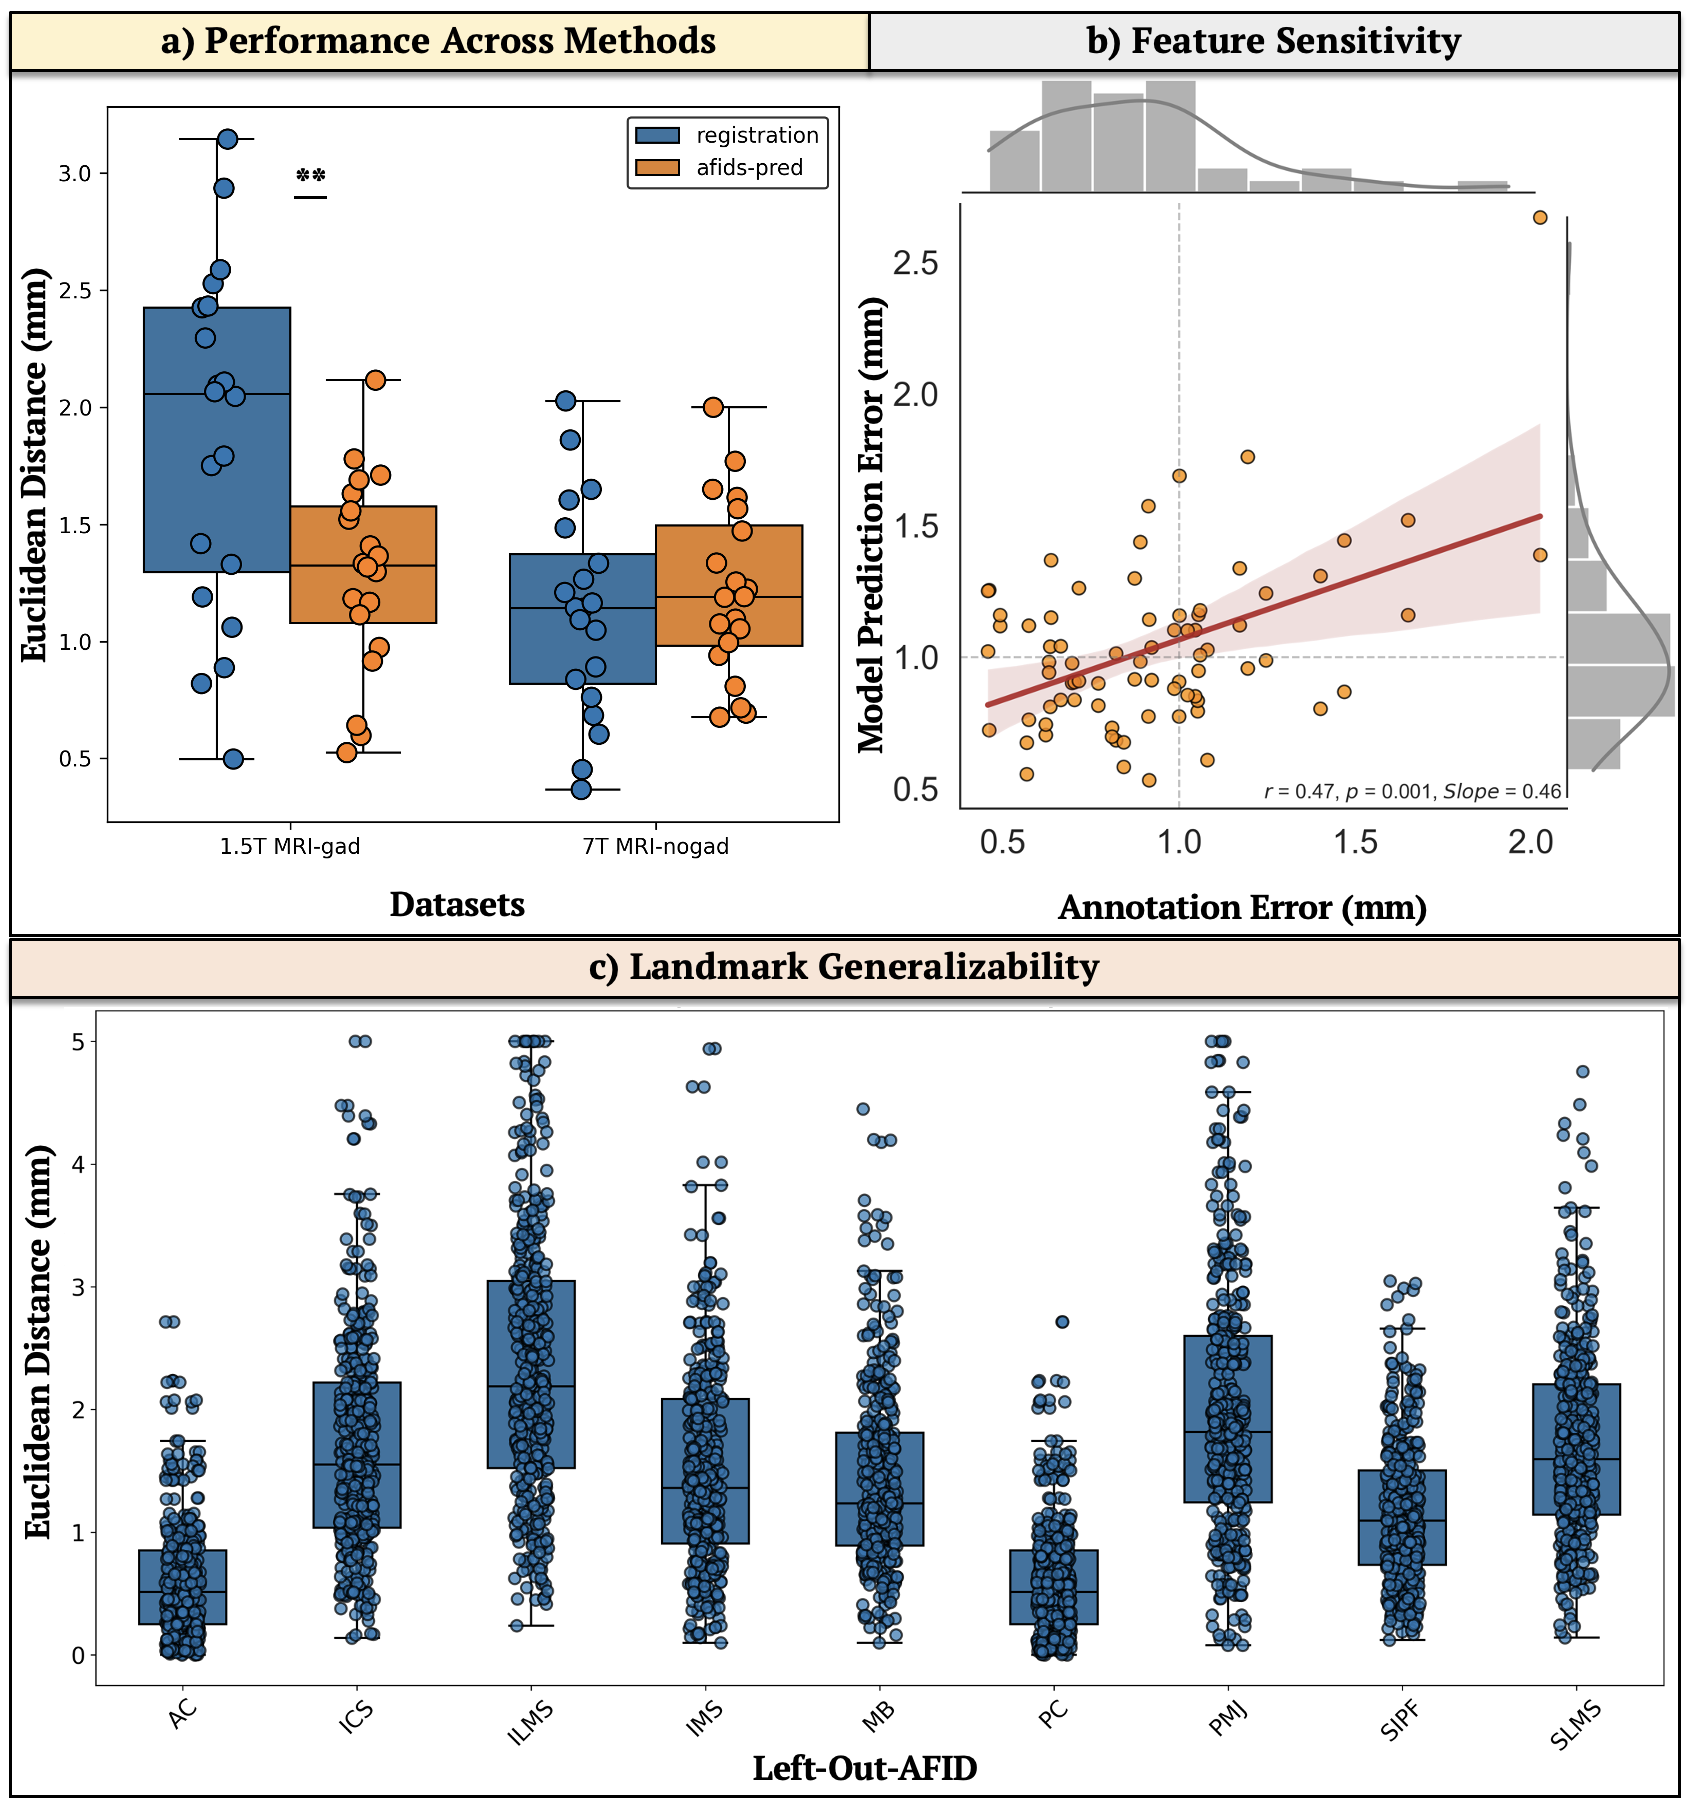
\includegraphics[width=1\linewidth]{figs/ch4_Figure_bench2.png}
    \caption{Model Benchmarking. a) Our model outperformed registration on the 1.5T MRI-gad dataset (p \(<\) 0.001) and performed just as well when using multispectral 7T MRI data (p \(>\) 0.1). b) AFID localization error was moderately linearly correlated with model performance (Pearson r = 0.47). c) Generalization to nine other midbrain landmarks.}
    \label{fig:ch4_Figure_bench}
\end{figure}

\textbf{Feature Importance and Augmentation:} To assess the influence of landmark annotation error on model performance, we examined the relationship between rater AFID localization error and ML model prediction error. A moderate correlation was observed (Pearson $r = 0.47$; $p < 0.01$), see Figure~\ref{fig:ch4_Figure_bench}b).

\textbf{Generalizability to Other Brain Landmarks:} To assess the broader applicability of our framework, we extended the localization approach to nine additional midbrain landmarks (see Figure~\ref{fig:ch4_Figure_bench}c). The model maintained high accuracy across these structures, achieving a median ED of 1.27~$\pm$~0.96~mm (IQR: 0.73–2.00).

\subsection{Clinical Use Cases}
We evaluated the functionality of our website using two illustrative DBS cases from our center (see Figure~\ref{fig:ch4_Figure_clincase}). In \textbf{Case 1}, we independently applied our framework to multimodal imaging data. The predictions were consistently within 1 mm across the following modalities: (1) 1.5-T MRI-gad, (2) 7-T T1w MRI, (3) 7T T2w MRI, and (4) contrast-enhanced CT. In \textbf{Case 2}, we demonstrated the application of our model to post-operative MRI from a DBS re-implantation case, highlighting its robustness in the presence of electrode artifacts that may complicate image-based localization methods.

\section{Discussion}
We demonstrated that coordinates of predefined brain landmarks can be leveraged to predict the coordinates of other surrounding brain regions with millimetric accuracy. By employing a coordinate-to-coordinate ML framework, our model is agnostic to MRI modality and resolution. Furthermore, we demonstrated that our model outperforms conventional methods when using challenging clinical-grade scans (e.g., 1.5-T MRI-gad) and performs just as well when using multispectral research-grade scans (i.e., 7-T MRI). Finally, we packaged this model in the form of a website, enabling its use in clinical and neuroimaging contexts.

\subsection{Rater Curated Data}
\textbf{AFID Annotations.} Previous AFID validation studies demonstrated millimetric localization in healthy \cite{Lau2019-eh} and clinical populations \cite{Abbass2022-lf}. The subset of 16 AFIDs in our ML framework were selected for their spatial proximity to the STN, sampling the morphology of the midbrain region. Although the complete AFIDs protocol (i.e., 32 AFIDs) typically requires 20–40 minutes following rater training, we anticipate a substantial reduction in annotation time due to the reduced number of AFIDs used here. To facilitate reproducibility and completeness, we provide a website embedded protocol tailored to the 16 AFIDs used in this work: \url{https://stereotaxy.afids.io}.
\begin{figure}[hbt!]
    \centering
    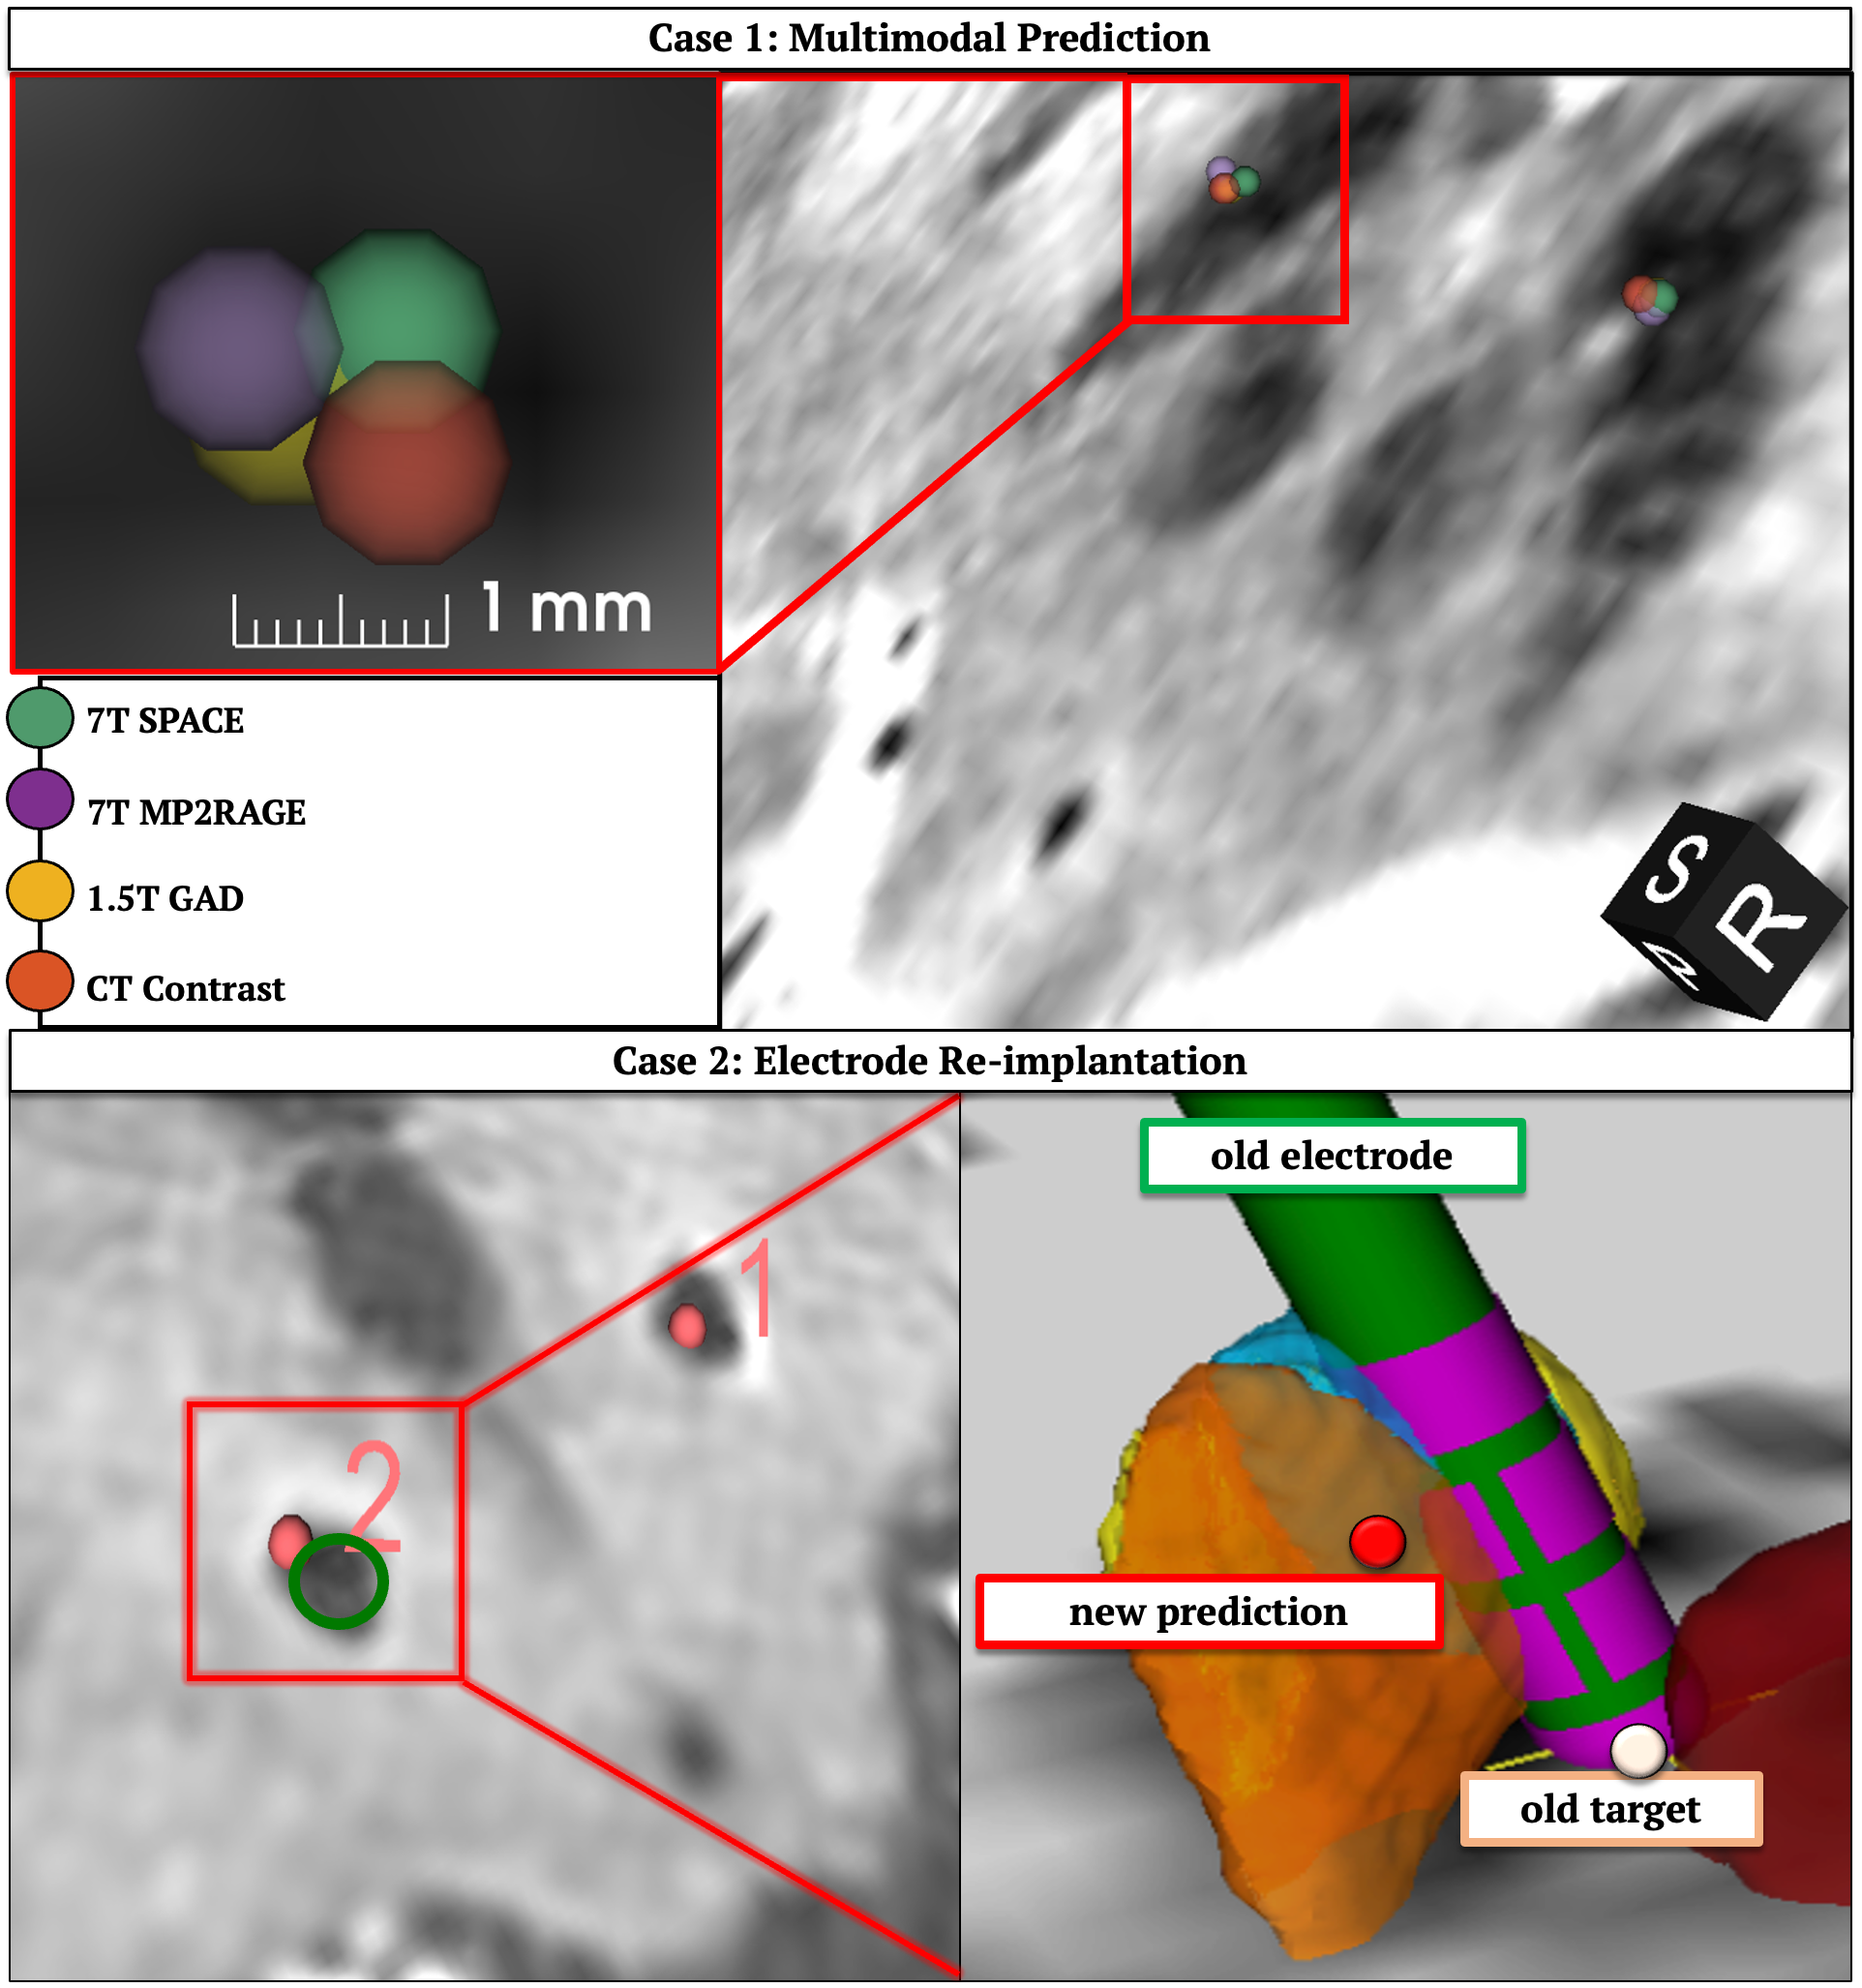
\includegraphics[width=1\linewidth]{figs/ch4_Figure_clincase.png}
    \caption{Clinical use cases. Case 1) Model prediction on multimodal neuroimaging data is within 1 mm of ground truth location as defined by expert raters on 7T-T2w MRI. All comparisons are made in anterior and posterior commissure space. Case 2) Model performance during a deep brain stimulation electrode re-implantation case using the postoperative MRI scan. Acquiring high-resolution imaging was not feasible due to the presence of electrodes}
    \label{fig:ch4_Figure_clincase}
\end{figure}

\newpage
\textbf{STN Annotations.} Inter-rater agreement for STN segmentation was strong, with a Dice similarity coefficient of \( 0.78 \pm 0.03 \). This is consistent with prior manual segmentation studies of the STN and nearby subcortical structures \cite{Camlidag2014-za,Miller2023-ct}. Prior work also highlighted that no statistically significant differences were found between left and right STN annotations \cite{Duchin2018-sv, Miller2023-ct}, justifying their combination in subsequent analyses. On average, the STN volume was reduced in the PD cohort relative to controls (\( 128.03 \pm 29.67 \text{ mm}^3 \) and \( 136.56 \pm 16.24 \text{ mm}^3 \), \( p = 0.047 \)). However, this volume difference did not remain statistically significant after Bonferroni correction. Prior studies reported conflicting findings, with some showing no significant difference in STN volume between PD and HC \cite{Alkemade2017-tt, Camlidag2014-za}, while others showing a reduction in the PD cohort \cite{Colpan2010-up, Patriat2020-cm}. We believe a meta-analytic approach is needed for more conclusive findings. Analysis of STN coordinates relative to the MCP revealed a significant inferior shift (i.e., z-axis) in PD patients compared to controls (\( p = 0.002 \)). This finding may support prior work reporting region-specific morphological changes associated with PD \cite{Kaya2019-wa}. Interestingly, previous work comparing STN coordinates between PD and essential tremor patients reported no significant differences \cite{Duchin2018-sv}; however, essential tremor may not serve as an appropriate baseline for comparison.

\subsection{Preliminary Analysis and PCA}
Our analysis demonstrates that brainstem AFIDs exhibit strong internal spatial correlations, consistent with prior reports of geometrical regularity in this region \cite{Perera2024-lq}. Structures such as the superior lateral mesencephalic sulcus (SLMS), superior interpeduncular fossa (SIPF), and mammillary bodies (MB) were tightly coupled along shared axes, suggesting conserved spatial organization may be driven by developmental and structural constraints \cite{Parraga2016-bl}. PCA supported this anatomical consistency, with the top five components capturing over 90\% of the variance in AFID coordinates. This high redundancy enables efficient dimensionality reduction for downstream ML applications, preserving anatomical information while reducing model complexity. Importantly, variance was broadly distributed across AFIDs rather than dominated by a few landmarks, reflecting coordinated spatial variation across regions. When correlating AFIDs with STN coordinates, SLMS ranked among the top predictors for all axes (\( r = 0.28\text{-}0.54 \)). The MB and SIPF also demonstrated strong associations (MB: \( r = 0.32\text{--}0.40 \); SIPF: \( r = 0.38\text{--}0.39 \)), highlighting the predictive value of midbrain and diencephalic landmarks. Taken together, these results support a coordinate-based localization approach, leveraging anatomical relationships to infer the position of brain targets.

\subsection{ML Model Performance}
Our model achieved a median localization error of \( 1.20 \pm 0.44\text{mm} \) (IQR: \( 0.84 - 1.52 \)) across all testing data. This performance is comparable to the localization variability of AFIDs themselves, previously reported to range from \( 0.36 \) to \( 1.68 \text{ mm} \) \cite{Lau2019-eh}. For context, a recent study reported an inter-rater centroid localization error of \( 1.90 \pm 1.07 \text{ mm} \) between two expert annotators \cite{Miller2023-ct}. A related coordinate-to-coordinate framework \cite{Engelhardt2021-zd} achieved a mean error of \( 1.33 \pm 1.64 \text{ mm} \); however, direct comparison is limited, as their target was the active contact of a DBS electrode rather than an anatomical structure. Notably, \cite{Guo2007-nf} benchmarked six STN targeting methods and found that a combined anatomical and functional approach yielded a localization error of \( 1.70 \pm 0.7 \text{ mm} \). Clinically, errors under \( 2 \text{ mm} \) are generally acceptable \cite{Kremer2023-if}, particularly when considering the typical stimulation volume of a DBS electrode.

\subsection{Model Generalizability and Comparisons}
\textbf{Validation Across Other Imaging Modalities.} This analysis was enabled by the use of paired datasets, allowing for direct comparison of predictions across modalities within the same subjects. Our framework’s accuracy was maintained across a range of imaging modalities. These findings align with prior work from our group, which established the feasibility of accurately localizing AFIDs across research-grade and clinical-grade MRI scans \cite{Taha2023-gd}. Importantly, comparisons were conducted in AC-PC space, which assumes that independent AFID placements across paired modalities result in equivalent transforms. This approach was necessary due to the lack of ground truth STN segmentations in both the 1.5-T MRI-gad and 3-T MRI datasets. Despite this potential source of error, our results revealed no statistically significant differences in predicted coordinates.

\textbf{Model Comparison and Performance Benchmarking.} We used the default registration pipeline in Lead-DBS to transform images from stereotactic space to native space. This pipeline employs rigorously optimized parameters \cite{Ewert2019-cc,Schonecker2009-xj} for diffeomorphic registration from Advanced Normalization Tools \cite{Avants2008-ek}. It also incorporates subcortical masks to refine deformation fields, enhancing registration accuracy at the STN and surrounding subcortical structures \cite{Ewert2019-cc, Schonecker2009-xj}. Our model statistically outperformed registration when using 1.5-T MRI-gad scans. MRI-gad scans are often considered a “lowest common denominator” scan employed for neurosurgical planning due to the combination of high spatial resolution and visualization of cerebral vasculature to ensure safe trajectories. However, the added contrast introduces bias during registration \cite{Abbass2022-lf, Abbass2025-el, Ogunsanya2024-uf}. Furthermore, our clinical images were of a lower resolution (i.e., \( 1.25 \times 1.25 \times 1.50 \) mm) which most likely hindered registration performance. Our model performed just as well as registration on multispectral 7-T MRI-nogad data. Prior work comprehensively addressed the added benefit of multispectral imaging \cite{Ewert2019-cc}. In this analysis, we employed sub-millimetric 7-T T1w and T2w MRI data, which represent an ideal and rigorous benchmark. Our model’s ability to match registration performance under these conditions highlights its potential utility in settings that lack access to 7-T MRI. To our knowledge, our analysis represented the first millimetric account of registration error on MRI-gad scans at the STN. Future investigations should focus on a more comprehensive account of two elements pertaining to registration: (1) isolating and accounting for the MRI-gad bias introduced during registration by employing paired data with identical pulse sequence parameters and (2) evaluating which set of multispectral data provides the best advantage during registration.

\textbf{Robustness to Annotation Variability.} Our model performance is, as expected, dependent on the accuracy of AFID localization. However, the relationship between model prediction error increases linearly with AFID localization error (e.g., with every 1 mm of annotation error, prediction accuracy declines by approximately 0.46 mm; see Figure \ref{fig:ch4_Figure_bench}b). We believe the robustness to annotation error came from various factors: (1) PCA on input features, which attenuates the impact of isotropic noise by prioritizing structured anatomical variance and down-weighting noisy, low-variance directions; (2) Redundancy among AFIDs, where overlapping spatial information allows the model to compensate for small errors in individual landmarks; and (3) Regularization, which reduces model sensitivity to noisy features by constraining coefficient magnitudes.

\textbf{Generalizability to Other Brain Landmarks.} Our framework maintained high millimetric localization accuracy across nine anatomically distinct landmarks. This finding supports the idea that spatial relationships captured from AFIDs enable localization of subcortical regions and can be applied to other DBS targets.

\subsection{Limitations and Future Directions}
A key limitation of our framework is its reliance on the accurate localization of AFIDs. However, prior studies have demonstrated that AFIDs can be placed reliably across diverse rater demographics and MRI modalities. Furthermore, our detailed open-access placement protocol is designed to make AFID localization more accessible and standardized for a wider user base. Importantly, for our primary use case in DBS, neurosurgeons are accustomed to localization of AFIDs such as the AC and PC as part of routine clinical workflows. Extending these established practices to a broader set of landmarks within the AFID framework is therefore both feasible and well-aligned with current surgical expertise.

Although our model localizes the STN center with millimetric accuracy, it is important to recognize that optimal DBS outcomes are typically achieved by targeting the subregions of the STN (e.g., dorsolateral STN in PD which corresponds to its motor functional territory). This spatial precision is crucial, as the true therapeutic substrate of DBS lies in modulating specific brain networks. In this work, we maintained an anatomically grounded framework as the STN center can be more objectively defined. However, our approach could be adapted to predict coordinates of sub-regions shown to have optimal therapeutic outcomes \cite{Hollunder2024-wc}. Such extensions would allow the model to bridge anatomical and functional targeting strategies, offering a path toward individualized and clinically informed neuromodulation planning.

Our current model is only geometry-based, relying on AFIDs without incorporating subject-level information that could enhance prediction accuracy or clinical relevance. Variables such as age, sex, diagnosis, disease severity, or even brain volume may further improve ML-driven localization accuracy. Future iterations of our framework could benefit from a hybrid approach, integrating demographic and clinical covariates alongside anatomical features to better tailor predictions to individual patients and potentially improve outcome prediction.

While DBS planning often involves implanting electrodes at predefined coordinates, this coordinate-based paradigm has limitations. In broader neuroscience contexts, many structures may not be fully captured by a single coordinate or point representation. Functional circuits, for instance, often span multiple anatomical boundaries, and their representation may be better suited to surface-based or tractography-informed models. Thus, while our current framework emphasizes precision within an anatomical coordinate system, future work may benefit from integrating volumetric, functional, or connectivity-based representations to holistically capture the complexity of brain structure–function relationships.
\newline
\section{Conclusions}
In summary, we validated a coordinate-to-coordinate regression framework for the localization of deep brain structures, and validated this framework on a common DBS target (i.e., STN). The model achieved millimetric precision, demonstrated strong generalizability across imaging modalities and additional subcortical landmarks, and outperformed conventional methods for brain structure localization on clinical-grade scans. Its robustness to moderate annotation variability and low computational overhead make it well-suited for integration into neurosurgical planning pipelines. To facilitate accessibility and reproducibility, we have deployed the model as a user-friendly web application and openly released all associated code and coordinate datasets.

